\chapter{Game semantics}
\label{chap:gamesem}

The aim of this chapter is to introduce game semantics. It starts with a history of game semantics and a presentation of the full abstraction problem for \pcf\ which has been solved using game semantics. It proceeds to introduce the basic notions of game
semantics and give a categorical interpretation of games. Finally we show how games are used to define a syntax-independent model of programming languages like \pcf\ and Idealized Algol (IA).

This chapter is largely based on the tutorial by Samson Abramsky on Game Semantics \citep{abramsky:game-semantics-tutorial}. Many
details and proofs will be omitted and we refer the reader to \cite{hylandong_pcf, abramsky94full} for a complete description of game semantics.

\section{History}

\subsection{Game semantics}

In the 1950s, Paul Lorenzen invented Game semantics as a new
approach to study semantics of intuitionistic logic \citep{lor61}.
In this setting, the notion of logical truth is modeled using game
theoretic concepts (mainly the existence of winning strategy).

Four decades later, game semantics is used to prove the full completeness of Multiplicative Linear Logic (MLL) \citep{abramsky92games,HO93a}. Shortly after, a connection between games and linear logic was established. Game semantics has then emerged as a new paradigm for the study of formal models for programming languages. The idea is to model the execution of a program as a game played by two protagonists. The Opponent represents the environment and the Proponent represents the system.
The meaning of the program is then modeled by a strategy for the Proponent.


Subsequently, these game-based model have been used to give a solution to the long-standing problem of ``Full abstraction of \pcf'' \citep{abramsky94full, hylandong_pcf,Nickau:lfcs94}.

Based on that major result, and in a more applied direction, games semantics has been used as a new tool for software verification \cite{ghicamccusker00}. This opened-up a new field called Algorithmic Game Semantics \citep{Abr02}.




\subsection{Model of programming languages}

Before the 1980s, there were many approaches to define models for programming languages. Among the successful ones, there were the axiomatic, operational and denotational semantics.
\begin{itemize}
\item Operational semantics gives a meaning to a program by describing the behaviour of a machine executing the program. It is defined formally
by giving a state transition system.
\item Axiomatic semantics defines the behaviour of the program through the use of axioms and is used to prove program correctness
by static analysis of the code of the program.
\item The denotational semantics approach consists in mapping a program to a mathematical structure
having good properties such as compositionality. This mapping is achieved by structural induction on the syntax of the program.
\end{itemize}

In the 1990s, three different independent research groups: Samson
Abramsky, Radhakrishnan Jagadeesan and Pasquale Malacaria
\citep{abramsky94full}, Martin Hyland and Luke Ong
\citep{hylandong_pcf} and Nickau \citep{Nickau:lfcs94} introduced
game semantics, a new kind of semantics, in order to solve a long
standing problem in the semanticists community -- finding a fully
abstract model for \pcf.

\subsection{The problem of full abstraction for \pcf}

\pcf\ is a simple programming language introduced in a classical
paper by Plotkin ``LCF considered as a programming language''
(\cite{DBLP:journals/tcs/Plotkin77}). \pcf\ is based on LCF, the
Logic of Computable Functions devised by Dana Scott in
\cite{scott_lcf}. It is a simply-typed lambda calculus extended with
arithmetic operators, conditional and recursion.

The problem of the Full Abstraction for \pcf\ goes back to the
1970s. In \citep{scott93}, Scott gave a model for \pcf\ based on
domain theory. This model gives a sound interpretation of
observational equivalence -- if two terms have the same domain
theoretic interpretation then they are observationally equivalent.
However the converse is not true -- there exist two \pcf\ terms
which are observationally equivalent but have different domain
theoretic denotations. As a result, we say that the model is not
fully abstract.

The key reason why the domain theoretic model of \pcf\ is not fully
abstract is that the parallel-or operator defined by the following
truth table
\begin{center}
\begin{tabular}{l|lll}
p-or  & $\bot$ & tt & ff \\ \hline
$\bot$ & $\bot$ & tt & $\bot$\\
tt & tt & tt & tt\\
ff & $\bot$ & tt & ff\\
\end{tabular}
\end{center}
is not definable as a \pcf\ term. It is possible to create two
different \pcf\ terms that always behave in the same way except when
applied to a term computing p-or. Since p-or is not definable in
\pcf, these two terms will have the same denotation. This implies
that the model is not fully abstract.


It is possible to patch \pcf\ by adding the operator p-or, the
resulting language ``\pcf+p-or'' becomes fully-abstracted by Scott
domain theoretic model \citep{DBLP:journals/tcs/Plotkin77}. The language we are now dealing with, however,
is strictly more powerful than
\pcf\ since it allows parallel execution of commands whereas \pcf\
only permits sequential execution.

Another approach involves the elimination of the undefinable
elements (like p-or) by strengthening the conditions on the function
used in the model. This approach has been followed by Berry in
\cite{berry-stable,gberry-thesis} where he gives a model based on
stable functions. Stable functions are a class of functions smaller
than the class of strict and continuous function. Unfortunately this
approach did not succeed.

Full abstract models for \pcf\ were found at the same time and independently by three research teams: Abramsky, Jagadeesan and Malacaria \citep{abramsky94full}, Hyland and Ong \citep{hylandong_pcf} and Nickau \citep{Nickau:lfcs94}. These three approaches are all based on game semantics.

The game semantics approach has then been adapted to other varieties of programming paradigms including languages with stores (Idealized Algol), call-by-value \citep{honda99gametheoretic,abramsky98callbyvalue} and call-by-name, general references \citep{DBLP:conf/lics/AbramskyHM98}, polymorphism
\citep{DBLP:journals/apal/AbramskyJ05}, control features
(continuation and exception), non determinism, concurrency. In all these cases, the game semantics model led to a syntax-independent fully abstract model of the corresponding language.

\section{Games}
\label{sec:catgames}

We now introduce formally the notion of game that will be used in
the following section to give a model of the programming languages
\pcf\ and Idealized Algol. The definitions are taken from
\cite{abramsky:game-semantics-tutorial, hylandong_pcf,
abramsky94full}.

The games we are interested in are two-players games. The players
are named O for Opponent and P for Proponent. The game played by O
and P is constrained by the \emph{arena}. The arena defines the
possible moves of the game. By analogy with real board games, the
arena represents the board together with the rules that tell players
how they can make their moves on the board. The analogy with board
game will not go beyond that. Instead, it is better to regard our
games as dialogs between two players: player O interviews player P.
P's goal is to answer the initial question asked by O. P can also
ask questions to O if he needs more precision about O's initial
question. Again, O can ask further question to P. This induces a
flow of questions and answers between O and P that can continue
possibly forever. In game semantics the attention is given to the
study of this flow of questions and answers, the notion of winner of
the game is not a concern.

\subsection{Arenas}


Our games have two kinds of moves -- the questions and the answers.
We also distinguish moves made by O and those made by P. An arena is
represented by a directed acyclic graph (DAG) whose nodes correspond
to question moves and leaves correspond to answer moves. It is
formally defined as follows.
\begin{definition}[Arena]
An arena is a structure $\langle M, \lambda, \vdash \rangle$ where:
\begin{itemize}
\item $M$ is the set of possible moves;
\item $(M,\vdash)$ is a directed acyclic graph;

\item $\lambda : M \rightarrow \{ O, P\} \times \{Q, A\}$ is a labelling function indicating whether a given move
    is a question or an answer and whether it can be played by O or P.

    $\lambda = [\lambda^{OP},\lambda^{QA}]$ where $\lambda^{OP} : M \rightarrow  \{ O, P\}$
    and $\lambda^{QA} : M \rightarrow  \{ Q, A\}$.

    \begin{itemize}
    \item If $\lambda^{OP} (m) = O$, we call $m$ an O-move otherwise $m$ is a P-move.
    $\lambda^{QA} (m) = Q$ indicates that $m$ is a question otherwise $m$ is an answer.

    \item a leaf $l$ of the DAG $(M,\vdash)$ satisfies $\lambda^{QA} (l) = A$ and a node
    $n$ satisfies $\lambda^{QA} (n) = Q$.
    \end{itemize}

\item The DAG $(M,\vdash)$ respects the following condition:
    \begin{itemize}
    \item[(e1)] The roots are O-moves: for any root $r$ of $(M,\vdash)$, $\lambda^{OP} (r) =
    O$;
    \item[(e2)] enablers are questions: $m \vdash n  \imp \lambda^{QA}(m) =
    Q$;
    % Or more succinctly, if we write $\dashv$ the relation $\vdash^-1$: $\lambda^{QA} \left( \dashv( (\lambda^{QA})^{-1}(\{A\}) ) \right) = \{ O \}$
    \item[(e3)] a player's move must be justified by a move played by the other player:
         $m\vdash n \imp \lambda^{OP}(m) \neq \lambda^{OP}(n)$.
    \end{itemize}
\end{itemize}
\end{definition}

For the sake of convenience we write the set $\{O,P\} \times
\{Q,A\}$ as $\{OQ,OA,PQ,PA\}$. $\overline{\lambda}$ denotes the
labelling function obtained from $\lambda$ after swapping players:
\begin{eqnarray*}
\overline{\lambda(m)} &=& OQ \iff \lambda(m) = PQ \\
\mbox{ and } \overline{\lambda(m)} &=& OA \iff \lambda(m) = PA
\end{eqnarray*}

The roots of the DAG $(M,\vdash)$ are called the \emph{initial moves}.
Other moves must be enabled by some other question move. The edges of the DAG induces the enabling relation between moves.

The simplest possible arena, written $\mathbf{1}$, is the arena with an empty set of moves.

\begin{example}[The flat arena]
\label{exmp:flatarena}

 Let $A$ be any countable set, then the flat arena over $A$
is defined to be the arena $\langle M, \lambda, \vdash \rangle$ such
that $M$ has one move $q$ with $\lambda(q) = OQ$ and for each
element in $A$, there is a corresponding move $a_i$ in $M$ with
$\lambda(a_i) = PA$ for some $i \in \nat$. The enabling relation
$\vdash$ is defined to be $\{ q \vdash a_i \ | i \in \nat \}$.
This arena is represented by the tree 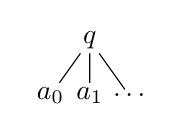
\begin{tikzpicture}[baseline=(root.base),level distance=7mm,inner ysep=0.5mm,sibling distance=5mm]
\node (root) {$q$}
child {node {$a_0$}}
child {node {$a_1$}}
child {node {$\ldots$}};
\end{tikzpicture}
 whose vertices represent the moves and edges represent the enabling relation. The flat arena over $\nat$ and $\mathbb{B}$ is written $\mathbf{int}$ and  $\mathbf{bool}$ respectively.
\end{example}

Once the arena has been defined, the bases of the game are set and the players have something to play with.
We now need to describe the state of the game, for that purpose
we introduce \emph{justified sequences of moves}:
\begin{definition}[Justified sequence of moves]
A justified sequence is a sequence of moves $s$ together with an
associated sequence of pointers. Any move $m$ in the sequence that
is not initial has a pointer that points to a previous move $n$ that
justifies it (i.e. $n \vdash m$).
\end{definition}
Since initial moves are all O-moves, the first move of a justified
sequence is necessarily an O-move

A justified sequence can be encoded as a sequence of pairs -- a pair
encodes an element of the sequence together with an index indicating
the position where the element points to.

The pointers of a justified sequence are represented with arrows.
The following is an example of justified sequence of moves:
$$\Pstr{ (q4){q^4}\ (q3-q4){q^3}\  (q2-q3){q^2}\ (q3b-q4){q^3}\ (q2b-q3b){q^2}\ (q1){q^1}\
}$$

Sequences of moves will be used to record the history of all the
moves that have been played.


\vspace{18pt} \emph{Notation:} we write $s t$ or sometimes $s \cdot
t$ to denote the sequences obtained by concatenating $s$ and $t$.
The empty sequence is written $\epsilon$. Given a sequence $s = m_1
\cdot m_2 \ldots m_n$ we write $s_{\leq m_i}$ for $m_1 \cdot m_2
\ldots m_i$, the prefix sequence of $s$ up to the move $m_i$. We
write $s_{< m_i}$ for $m_1 \cdot m_2 \ldots m_{i-1}$.


A justified sequence has two particular subsequences called the P-view and the O-view
of the sequence. The idea is that a view describes the local context
of the game. Here is the formal definition:
\begin{definition}[View]
Given a justified sequence of moves $s$, we define the proponent view (P-view) written $\pview{s}$ by induction:
\begin{align*}
\pview{\epsilon} &= \epsilon, \\
\pview{s \cdot m} &= \pview{s} \cdot \ m && \mbox{ if $m$ is a P-move}, \\
\pview{s \cdot m} &= m && \mbox{ if $m$ is initial (O-move) }, \\
\pview{ \Pstr{ s \cdot (m){m} \cdot t \cdot (n-m){n}} } &=
     \Pstr{ \pview{s} \cdot (m2){m} \cdot (n2-m2){n}} && \mbox{ if $n$ is a non initial O-move
 }.
\end{align*}
The O-view $\oview{s}$ is defined similarly:
\begin{align*}
\oview{\epsilon} &= \epsilon, \\
\oview{s \cdot m} &= \oview{s} \cdot \ m && \mbox{ if $m$ is a O-move}, \\
\oview{ \Pstr{ s \cdot (m){m} \cdot t \cdot (n-m){n} } } &=
\Pstr{ \pview{s} \cdot (m2){m} \cdot (n2-m2){n} } && \mbox{ if $n$ is a P-move
 }.
\end{align*}
\end{definition}


\subsection{Games}

Not all justified sequences will be of interest for the
games that we will use. We call \emph{legal position} justified
sequences that satisfy two additional conditions: alternation and
visibility. Alternation says that players O and P play
alternatively. Visibility expresses that each non-initial move is
justified by a move situated in the local context at that point.
The visibility condition gives some coherence to the
justification pointers of the sequence.

\begin{definition}[Legal position]
A legal position is a justified sequence of move $s$ respecting the following constraints:
\begin{itemize}
\item \emph{Alternation}: For any subsequence $m \cdot n$ of $s$, $\lambda^{OP}(m) \neq \lambda^{OP}(n)$.
\item \emph{Visibility}: For any subsequence $t m$ of $s$ where $m$ is not initial, if $m$ is a P-move then $m$ points to a move in $\pview{s}$
and if $m$ is a O-move then $m$ points to a move in $\oview{s}$.
\end{itemize}
The set of legal position of an arena $A$ is denoted by $L_A$.
\end{definition}

We say that a move $n$ is hereditarily justified by a move $m$ if there is a sequence of move
$m_1, \ldots, m_q$ such that:
$$ m \vdash m_1 \vdash m_2 \vdash \ldots m_q \vdash n$$
If a move has no justification pointer, we says that it is an
\emph{initial move} (in that case it must be a root of the DAG of the arena).

Suppose that $n$ is an occurrence of a move in the sequence $s$ then
$s \filter n$ denotes the subsequence of $s$ containing all
the moves hereditarily justified by $n$. Similarly, $s
\filter I$ denotes the subsequence of $s$ containing all the
moves hereditarily justified by moves in $I$.

\begin{definition}[Game]
A game is a structure $\langle M, \lambda, \vdash, P \rangle$ such that
\begin{itemize}
\item $ \langle M, \lambda, \vdash \rangle$ is an arena;
\item $P$ is called the set of valid positions, it is:
    \begin{itemize}
    \item a non-empty prefix closed subset of the set of legal
    positions,
    \item closed by initial hereditary projection: if $s$ is a valid position then for any set $I$ of occurrences of initial moves
    in $s$, $s\filter I$ is also a valid position.
    \end{itemize}
\end{itemize}
\end{definition}

\begin{example}Consider the flat arena  $\mathbf{int}$.
The set of valid position $P = \{ \epsilon, q \} \union \{ q \cdot
a_i \ | i \in \nat \}$ defines a game on the arena $\mathbf{int}$.
\end{example}

\subsection{Constructions on games}
\label{sec:gameconstruction}

We now define game constructors that will be useful later on.

Consider the two functions $f : A \rightarrow C$ and $g : B
\rightarrow C$, we write $[f,g]$ to denote the pairing of $f$ and
$g$ defined on the direct sum $A + B$. Given a game $A$ with a set
of moves $M_A$, we use the projection operator $s \filter A$ to
denote the subsequence of $s$ consisting of all moves in $M_A$.
Although this notation conflicts with the hereditary projection
operator, it should not cause any confusion.

\subsubsection{Tensor product}
Given two games $A$ and $B$ we define the tensor product constructor
$A \otimes B$ as follows:
\begin{eqnarray*}
  M_{A \otimes B} &=& M_A + M_B \\
  \lambda_{A\otimes B} &=& [\lambda_A,\lambda_B] \\
  \vdash_{A\otimes B} & = & \vdash_{A}\ \union\ \vdash_{B} \\
  P_{A\otimes B} & = & \{ s \in L_{A\otimes B} | s \filter A \in P_A \wedge s \filter B \in P_B  \}.
\end{eqnarray*}

In particular,  $n$ is initial in $A\otimes B$ if and only if $n$ is
initial in A or B. And $m \vdash_{A\otimes B} n$  holds if and only if $m
\vdash_{A} n$ or $m \vdash_{B} n$ holds.

\subsubsection{Function space}
The game $A \multimap B$ is defined as follows:
\begin{eqnarray*}
  M_{A \multimap B} &=& M_A + M_B \\
  \lambda_{A\multimap B} &=& [\overline{\lambda_A},\lambda_B] \\
  \vdash_{A\multimap B} & = & \vdash_{A}\ \union\ \vdash_{B}\ \union\  \{ (m,n) \ |\ m \mbox{ initial in } B \wedge n \mbox{ initial in } A \} \\
  P_{A\otimes B} & = & \{ s \in L_{A\otimes B} | s \filter A \in P_A \wedge s \filter B \in P_B  \}.
\end{eqnarray*}

Graphically if we draw a triangle to represent an arena $A$ then the
arena for $A \multimap B$ is represented as:
\begin{center}
\begin{tikzpicture}[baseline=(A.base),inner ysep=0.5mm,shape border rotate=90, isosceles triangle]
\path  node[draw] (A)  {$B$}
(-1.5cm,-0.7cm) node[draw] (B) {$A$} ;
\path (A.north) edge (B.north);
\end{tikzpicture}
\end{center}



\subsubsection{Cartesian product}
The game $A \& B$ is defined as follows:
\begin{eqnarray*}
  M_{A \& B} &=& M_A + M_B \\
  \lambda_{A\& B} &=& [\lambda_A,\lambda_B] \\
  \vdash_{A\& B} & = & \vdash_{A}\ \union\ \vdash_{B} \\
  P_{A\& B} & = & \{ s \in L_{A\otimes B} | s \filter A \in P_A \wedge s \ \filter B = \epsilon  \} \\
        &&   \union \{ s \in L_{A\otimes B} | s \filter A \in P_B \wedge s \ \filter A = \epsilon  \}.
\end{eqnarray*}

Note that a play of the game $A \& B$ is either a play of $A$ or a
play of $B$, whereas a play of the game $A \otimes B$ may be an
interleaving of plays on $A$ and plays on $B$.

\subsection{Representation of plays}

Plays of the game are usually represented in a table diagram. The
columns of the table correspond to the different components of the
arena and each row corresponds to one move in the play. The first
row always represents an O-move, this is because O is the only
player who can open a game (since roots of the arena are O-moves).

For example the play
$$\Pstr{ (q1){q}\
 (q2-q1){q}
 \ (a2-q2){8}
\  (a1-q1){12}}$$ on the game $\textbf{int} \multimap
\textbf{int} $ is represented by the following diagram:
\begin{center}
\begin{tabular}{cccc}
\textbf{int} & $\imp$ & \textbf{int} & \\
&& q & O\\
q  &&& P\\
8  &&& O\\
&& 12 & P
\end{tabular}
\end{center}

When it is necessary, the justification pointers of the play are
also shown on the diagram.


\subsection{Strategy}

During a game, the player who has to play may have several choices
for his next move. A strategy is a guide telling the player which move to make when the
game is in a given position. There is no notion of winning strategy since this is
not relevant for the games that we are considering.

\subsubsection{Definition}
Formally, a strategy is a partial function mapping legal positions
where P has to play to P-moves.
\begin{definition}[Strategy]
\label{dfn:strategy}
A strategy for player P on a given game $\langle M, \lambda, \vdash, P \rangle$ is a
non-empty set of even-length positions from $P$ such that:
\begin{enumerate}
\item if $sab \in \sigma$ then $s \in \sigma$ (\emph{no unreachable
position});
\item if $sab, sac \in \sigma$ then $b = c$  and $b$ has the same justifier as
$c$ (\emph{determinacy}).
\end{enumerate}
\end{definition}

The idea is that the presence of the even-length sequence $s a b$ in
$\sigma$ tells the player P that whenever the game is in position
$s$ and player O plays the move $a$ then it must respond by playing
the move $b$.

The first condition ensures that the strategy $\sigma$ only
considers positions that the strategy itself could have led to in a
previous move. The second condition in the definition requires that
this choice of move is deterministic (i.e. there is a function $f$
from the set of odd length position to the set of moves $M$ such
that $f(s a) = b$).


For any game $A$, the smallest possible strategy is called the
\emph{empty strategy} and written $\bot$. It is formally defined by
$\{ \epsilon \}$, which corresponds to a strategy that never
responds.


\begin{remark}
\label{rem:atlern_strategy} There is an alternative definition of a
strategy. If we regard a strategy as an appropriated sub-tree of the
game tree then it can be represented as the collection of all paths
in this sub-tree, that is to say a certain prefix-closed set (as
opposed to the \emph{even-length prefix}-closed set of the above
definition).

If $\sigma$ denotes a strategy in the sense of definition \ref{dfn:strategy} then the corresponding strategy in the alternative definition would be
$\sigma \union \textsf{dom}(\sigma)$ where
$$\textsf{dom}(\sigma) = \{ sa \in P_A^{odd} | \exists b . sab \in \sigma \}.$$
\end{remark}


\subsubsection{Copy-cat strategy}

For any arena $A$ there is a strategy on the game $A \multimap A$
called the \emph{copy-cat strategy}. We write $A_1$ and $A_2$ to
denote the first and second copies of the arena $A$ in the game $A
\multimap A$. If $A$ is the arena $A_1$ then $A^\perp$ denotes the
arena $A_2$ and reciprocally.

Let $A$ be one of the arena $A_1$ or $A_2$. The copy-cat strategy
operates as follows: whenever P has to respond to an O-move played
in $A$, it first replicates this move into the arena $A^{\perp}$.
$O$ then responds in $A^{\perp}$ and finally $P$ replicates O's
response back to $A$.


More formally, the copy-cat strategy is defined by:
$$ \textsf{id}_A = \{ s \in P^{\textsf{even}}_{A \multimap A} \ | \ \forall t \sqsubseteq^{\textsf{even}} s\ .\ t \filter A_1 = t \filter A_2 \}$$
where $P^{\textsf{even}}_A$ denotes the set of valid positions of
even length in the game $A$ and $t \sqsubseteq^{\textsf{even}} s$
denotes that $t$ is an even length prefix of $s$.

The copy-cat strategy is also called \emph{identity strategy} since
it is the identity for strategy composition as we will see in the
next paragraph.

\begin{example} The copy-cat strategy on $\textbf{int}$ is given by the following generic play:
$$\begin{array}{ccc}
\textbf{int} & \imp & \textbf{int} \\
&& q\\
q \\
n \\
&& n
\end{array}
$$
Note that we introduced this type of diagram in the first place in
order to represent plays but, as we can see here, whenever the
represented play is general enough, the diagram can be used to
represent strategies.

The copy-cat strategy on $\textbf{int} \imp \textbf{int}$ is given
by the following diagram:
$$\begin{array}{ccccccc}
(\textbf{int} & \imp & \textbf{int}) & \imp & (\textbf{int} & \imp & \textbf{int}) \\
&&&& && q\\
&& q\\
q \\
&&&& q \\
&&&& m \\
m\\
&& n \\
&&&& && n
\end{array}$$
\end{example}

\subsubsection{Composition}

It is well-known that any model of the simply-typed lambda-calculus
is a cartesian closed category \citep{CroleRL:catt}. Games are used
to give a fully-abstract model of \pcf\ -- an extended simply-typed
lambda calculus -- therefore the game model should fit into a
cartesian closed category. This category will have games as objects
and strategies as morphisms. In a category, morphisms should be able
to compose together, therefore there should be an appropriate notion
of strategy composition.

In the following section we will show how strategies can be used to
represent programs. A remarkable feature of the game model, called
compositionality, is that obtaining the model of a composed program
boils down to composing the strategies of the composing programs.
Composition of strategies is therefore an essential feature of game
semantics.


The way composition is defined for strategies is similar to
``parallel composition plus hiding'' in the trace semantics of CSP
\citep{hoare_csp}. Consider two strategies $\sigma : A \multimap B$
and $\tau : B \multimap C$ that we wish to compose. For any sequence
of moves $u$ on three arenas $A$, $B$, $C$, we call projection of
$s$ on the game $A \multimap B$ and we write $u \filter A,B$
for the subsequence of $s$ obtained by removing from $u$ the moves
in $C$ and pointers to moves in $C$. The projection on $B \multimap
C$ is defined similarly.

The definition of the projection on $A \multimap B$ differs
slightly: $u \filter A,C$ is the subsequence of $u$
consisting of the moves from $A$ and $C$ with some additional
pointers. We add a pointer from $a \in A$ to $c\in C$ whenever $a$
points to some move $b \in B$ itself pointing to $c$. All the
pointers to moves in $B$ are removed.


First we remark that for a given legal position $s$ in the game $A
\multimap C$, there is what is called an \emph{uncovering} of $s$.
The uncovering of $s$ is the maximal justified sequence of moves $u$
from the games $A$, $B$ and $C$ such that:
\begin{itemize}
\item The sequence $s$, considered as a pointer-less sequence, is a subsequence of
$u$;
\item the projection of $u$ on the game $A \multimap B$ belongs to the
strategy $\sigma$;
\item the projection of $u$ on the game $B \multimap C$ belongs
to the strategy $\tau$;
\item and the projection of $u$ on the game $A \multimap C$ is a subsequence of $s$ (here the term ``subsequence'' refers to the sequence of nodes together with the auxiliary sequence of pointers).
\end{itemize}
This uncovering, written $uncover(s, \sigma, \tau)$, is
defined uniquely for given strategies $\sigma$, $\tau$ and legal
position $s$ (this is proved in part II of \cite{hylandong_pcf}).

We define $\sigma \| \tau $ to be the set of uncovering of legal
positions in $A \multimap C$:
$$ \sigma \| \tau = \{ uncover(s, \sigma, \tau) \ | \ s \mbox{ is a legal position in } A \multimap C \}$$

The composition of $\sigma$ and $\tau$ is defined to be the set of
projections of uncovering of legal positions in $A \multimap C$:

\begin{definition}[Strategy composition]
Let $\sigma : A \multimap B$ and  $\tau : B \multimap C$ be two
strategies. We define $\sigma ; \tau$ to be:
$$ \sigma ; \tau = \{ u \filter A,C \ | \ u \in \sigma \|
\tau \}$$
\end{definition}

It can be verified that composition is well-defined and associative \citep{hylandong_pcf} and that the copy-cat strategy $\textsf{id}_A$ is the identity for composition.

\subsubsection{Constraint on strategies}

Different classes of strategies will be considered depending on the
features of the language that we want to model. Here is a list of
common restrictions that we will consider:
\begin{itemize}
\item \emph{Well-bracketing:}
We call \emph{pending question} the last question in a sequence that has not been answered.
A strategy $\sigma$ is well-bracketed if for every play $s \cdot m \in \sigma$ where $m$ is an answer, $m$ points to the pending question in $s$.

\item \emph{History-free strategies:} a strategy is history-free if the Proponent's move at any position of the game where he has to play
is determined by the last move of the Opponent. In other words, the
history prior to the last move is ignored by the Proponent when
deciding how to respond.

\item \emph{History-sensitive strategies:} The Proponent follows a history-sensitive strategy if he needs to have access to the full
history of the moves in order to decide which move to make.

\item \emph{Innocence:} a strategy is innocent if the determination of the Proponent's move depends
only on a restricted view of the history of the play, mainly the
P-view at that point. Such strategies can be specified by a partial
function mapping P-views to P-moves called the \emph{view function}.
However not every partial function from P-views to P-moves gives
rise to an innocent strategy (a sufficient condition is given in
\cite{hylandong_pcf}).
\end{itemize}

The formal definition of innocence follows:
\begin{definition}[Innocence]
Given positions $sab, ta \in L_A$ where $sab$ has even length and
$\pview{sa} = \pview{ta}$, there is a unique extension of $ta$ by
the move $b$ together with a justification pointer such that
$\pview{sab} = \pview{tab}$. We write this extension
$\textsf{match}(sab,ta)$.

The strategy $\sigma:A$ is \emph{innocent} if and only if:
$$ \left(
     \begin{array}{c}
       \pview{sa} = \pview{ta} \\
       sab \in \sigma \\
       t\in \sigma \wedge ta \in P_A \\
     \end{array}
   \right)
\quad \imp\quad  \textsf{match}(sab,ta) \in \sigma$$

\end{definition}


\subsection{Categorical interpretation}

In this section we recall some results about the categorical
representation of games. These results with complete details and
proofs can be found in \cite{McC96b,hylandong_pcf,abramsky94full}.
We refer the reader to \cite{CroleRL:catt} for more information
about category theory.

We consider the category $\mathcal{G}$ whose objects are games and morphisms are
strategies. A morphism from $A$ to $B$ is a strategy on the game $A \multimap B$.

Three other sub-categories of $\mathcal{G}$ are considered, each of
them corresponds to some restriction on strategies: $\mathcal{G}_i$
is the sub-category of $\mathcal{G}$ whose morphisms are the
innocent strategies, $\mathcal{G}_b$ has only the well-bracketed
strategies and $\mathcal{G}_{ib}$ has the innocent and
well-bracketed strategies.

\begin{proposition}
$\mathcal{G}$, $\mathcal{G}_i$, $\mathcal{G}_b$ and $\mathcal{G}_{ib}$ are categories.
\end{proposition}

Proving this requires us to prove that composition of strategies is
well-defined, associative, has a unit (the copy-cat strategy),
preserves innocence and well-bracketedness. See
\cite{hylandong_pcf,abramsky94full} for a proof.


\subsubsection{Monoidal structure}

We have already defined the tensor product on games in section
\ref{sec:gameconstruction}. We now define the corresponding
transformation on morphisms. Given two strategies $\sigma : A
\multimap B$ and $\tau : C \multimap D$ the strategy $\sigma \otimes
\tau : (A \otimes C) \multimap (B\otimes D)$ is defined by:
$$ \sigma \otimes \tau = \{ s \in L_{A \otimes C \multimap B\otimes D} \ s \filter A,B \in \sigma
\wedge s \filter C,D \in \tau \}$$

It can be shown that the tensor product is associative, commutative
and has $I = \langle \emptyset, \emptyset,\emptyset, \{ \epsilon \}
\rangle $ as identity. Hence the game category $\mathcal{G}$ is a
symmetric monoidal category. Moreover $\mathcal{G}_i$ and
$\mathcal{G}_b$ are sub-symmetric monoidal categories of
$\mathcal{G}$, and $\mathcal{G}_{ib}$ is a sub-symmetric monoidal
category of $\mathcal{G}_i$, $\mathcal{G}_b$ and $\mathcal{G}$.

\subsubsection{Closed structure}

Given the games $A$, $B$ and $C$, we can transform strategies on $A\otimes B \multimap C$ to
strategies on $A \multimap (B \multimap C)$ by retagging the moves to the appropriate arenas. This transformation
defines an isomorphism written $\Lambda_B$ and called currying. Therefore the hom-set $\mathcal{G}(A\otimes B, C)$ is isomorphic to the hom-set
$\mathcal{G}(A,B\multimap C)$ which makes $\mathcal{G}$ an autonomous (i.e. symmetric monoidal closed) category.

We write $ev_{A,B} : (A \multimap B) \otimes A \rightarrow B$ to denote the \emph{evaluation strategy} obtained by uncurrying the
identity map on $A \rightarrow B$. $ev_{A,B}$ is in fact the copycat strategy for the game
$(A \multimap B) \otimes A \rightarrow B$.

$\mathcal{G}_i$ and  $\mathcal{G}_b$ are sub-autonomous categories of $\mathcal{G}$,
and $\mathcal{G}_{ib}$ is a sub-autonomous category of $\mathcal{G}_i$, $\mathcal{G}_b$ and
$\mathcal{G}$.

\subsubsection{Cartesian product}
The cartesian product defined in section \ref{sec:gameconstruction} is indeed a cartesian product in the category
$\mathcal{G}$, $\mathcal{G}_i$, $\mathcal{G}_b$ and $\mathcal{G}_{ib}$.

The projections $\pi_1:A \& B \rightarrow A$ and $\pi_1:A \& B
\rightarrow B$ are given by the obvious copy-cat strategies. Given
two category morphisms $\sigma :C \rightarrow A$ and $\tau : C
\rightarrow B$, the pairing function $\langle \sigma, \tau \rangle :
C \rightarrow A \& B$ is given by:
\begin{eqnarray*}
\langle \sigma, \tau \rangle &=& \{ s \in L_{C\multimap A\&B} \ | \ s \filter C,A \in \sigma \wedge s \filter B = \epsilon  \} \\
&\union& \{ s \in L_{C\multimap A\&B} \ | \ s \filter C,B \in \tau \wedge s \filter A = \epsilon  \}
\end{eqnarray*}

\subsubsection{Cartesian closed structure}
Defining the cartesian product is not enough to turn $\mathcal{G}$
into a cartesian closed category : we also need to define a terminal
object $I$ and the exponential construct $A \imp B$ for any two
games $A$ and $B$. In fact, this cannot be done in the current
category $\mathcal{G}$ and we have to move on to another category of
games written $\mathcal{C}$ whose objects and morphisms are certain
sub-classes of games and strategies.

Before defining the category $\mathcal{C}$ we need to introduce some
definitions.


For any game $A$ we define the exponential game denoted by $!A$. The
game $!A$ corresponds to a repeated version of the game $A$. Plays
of $!A$ are interleavings of plays of $A$. It is defined as follows:
\begin{eqnarray*}
  M_{!A} &=& M_A \\
  \lambda_{!A} &=& \lambda_A \\
  \vdash_{!A} & = & \vdash_{A} \\
  P_{!A} & = & \{ s \in L_{!A} | \mbox{ for each initial move $m$, } s \filter m \in P_A \}
\end{eqnarray*}
The following equalities hold:
\begin{eqnarray*}
  !(A \& B) &=& !A \otimes !B\\
  I &=& !I
\end{eqnarray*}

\begin{definition}[Well-opened games]
A game $A$ is well-opened if for any position $s \in P_A$ the only initial move is the first
one.
\end{definition}

Well-opened games have single thread of dialog. They can be turned
into games with multiple-thread of dialog using the promotion
operator:

\begin{definition}[Promotion]
Consider a well-opened game $B$. Given a strategy on ${!A} \multimap
B$, we define its promotion $\sigma^\dagger : {!A} \multimap {!B}$
to be the strategy which plays several copies of $\sigma$. It is
formally defined by:
$$ \sigma^\dagger = \{ s \in L_{{!A} \multimap !B} \ | \ \mbox{ for all initial $m$, } s \filter m \in \sigma  \}.$$
\end{definition}

It can be shown that promotion is well-defined (it is indeed a strategy) and that it preserves innocence and
well-bracketedness.


We now introduce the category of well-opened games.
\begin{definition}[Category of well-opened games]
The category $\mathcal{C}$ of well-opened games is defined as
follows:
\begin{enumerate}
\item The objects are the well-opened games,
\item a morphism $\sigma : A \rightarrow B$ is a strategy for the game $!A \multimap B$,
\item the identity map for $A$ is the copy-cat strategy on $!A \multimap A$ (which is well-defined for well-opened games).
It is called dereliction, denoted by
$\textsf{der}_A$ and defined formally by:
$$ \textsf{der}_A = \{ s \in P^{\textsf{even}}_{{!A} \multimap A} \ | \ \forall t \sqsubseteq^{\textsf{even}} s \ . \ t \filter {!A} = t \filter A \},$$
\item composition of morphisms $\sigma : {!A} \multimap B$ and $\tau : {!B} \multimap C$
denoted by $\sigma \fatsemi \tau : {!A} \multimap C$ is defined as $\sigma^\dagger;\tau$.
\end{enumerate}
\end{definition}
$\mathcal{C}$ is a well-defined category and the three sub-categories
$\mathcal{C}_i$, $\mathcal{C}_b$, $\mathcal{C}_{ib}$ corresponding to sub-category
with innocent strategies, well-bracketed strategies and innocent and well-bracketed strategies respectively.


The category $\mathcal{C}$ has a terminal object $I$, for any two games $A$ and $B$ a product $A \& B$ and
an exponential $A \imp B$ defined to be $!A \multimap B$. The hom-sets $\mathcal{C}(A \& B,C)$ and
$\mathcal{C}(A,!B \multimap C)$ are isomorphic. Indeed:
\begin{eqnarray*}
\mathcal{C}(A\& B,C) &=& \mathcal{G}(!(A\& B),C) \\
&=& \mathcal{G}({!A}\otimes {!B},C) \\
&\cong& \mathcal{G}({!A}, {!B} \multimap C) \qquad  \mbox{($\mathcal{G}$ is a closed monoidal category)}\\
&=& \mathcal{C}(A, {!B} \multimap C)
\end{eqnarray*}
Hence $\mathcal{C}$ is a cartesian closed category. Moreover $\mathcal{C}_i$ and $\mathcal{C}_b$
are sub-cartesian closed caterogies of $\mathcal{C}$ and $\mathcal{C}_{ib}$ is as sub-cartesian closed category
of each of $\mathcal{C}$, $\mathcal{C}_i$ and $\mathcal{C}_b$.





\subsubsection{Order enrichment}

Strategies can be ordered using the inclusion ordering. Under this
ordering, the set of strategies on a given game $A$ is a pointed
directed complete partial order : the least upper bound is given by
the set-theoretic union and the least element is the empty strategy
$\{ \epsilon \}$.

Moreover all the operators on strategies that we have defined so far
(composition, tensor product, ...) are continuous. Hence the
categories $\mathcal{C}$ and $\mathcal{G}$ are cpo-enriched.

This property will prove to be useful when it comes to modeling
programming languages with recursion such as \pcf.


\subsubsection{Intrinsic preorder}

We now define a pre-ordering on strategies. The following definition
is valid in any of the categories $\mathcal{C}$, $\mathcal{C}_i$,
$\mathcal{C}_b$, $\mathcal{C}_{ib}$.

Let $\Sigma$ be the game with a single question $q$ and single
answer $a$. There are only two strategies on $\Sigma$: $\bot = \{
\epsilon \}$ and $\top = \{ \epsilon, q a \}$ which are both
innocent and well-bracketed. These strategies are used to test
strategies. For any strategy $\sigma : {\bf 1} \rightarrow A$ and
for any test strategy $\alpha : A \rightarrow \Sigma$ we say that
$\sigma$ passes the test $\alpha$ if $\sigma \fatsemi \alpha =
\top$.

The intrinsic preorder, written $\lesssim$, is defined as follows:
for any strategy $\sigma,\tau$ on the game $A$, $\sigma \lesssim
\tau$ if $\tau$ passes all the test passed by $\sigma$. Formally:
$$ \sigma \lesssim \tau \quad \iff \quad \forall \alpha : A \rightarrow \Sigma. \sigma \fatsemi \tau = \top \imp \tau \fatsemi \alpha = \top$$

One can check that the relation $\lesssim$ is indeed a preorder on
the set of strategies of the considered category. This preorder
defines classes of equivalence. Two strategies are in the same
equivalence class if no test can distinguish them. The quotiented
category is written $\bf C/\lesssim$ where $\bf C$ ranges over $\{
\mathcal{C}_i, \mathcal{C}_i, \mathcal{C}_b, \mathcal{C}_{ib} \}$.

Later on we will state the full abstraction of the game semantics model of \pcf. This result will
be proved in the quotiented category.

\subsection{Pointers are superfluous for games on arenas of order 2}

For any legal justified sequence of moves $s$, we write $?(s)$ for
the subsequence of $s$ obtained by keeping only the unanswered
questions in $s$. It is easy to check that if $s$ satisfies
alternation then $?(s)$ also satisfies alternation.

\begin{lemma}
  If $s\cdot q$ is a legal position (i.e. justified sequence satisfying visibility and alternation) satisfying
    well-bracketing where $q$ is a non-initial question then $q$ points in $?(s)$.
\end{lemma}
\begin{proof}
    By induction on the length of $s \cdot q$. The base case $s=\epsilon$ is trivial.
    Let $s = s\cdot q$, where $q$ is not initial.

    Suppose $q$ is a P-move. We prove that $q$ cannot point to an O-question that has been answered.
    Suppose that an O-move $q'$ occurs before $q$ and is answered by the move $a$ also occurring before $q$.
    Then we have $s = s_1 \cdot q'^O \cdot s_2 \cdot a^P \cdot s_3 \cdot q^P$ where $a$ is justified by $q'$.
    $a$ is not in the P-view $\pview{s_{<q}}$. Indeed this would imply that some O-move occurring in $s_3$ points to $a$, but this is impossible
    since answer moves are not enablers. Hence the move $a$ must be situated underneath an O-to-P link. Let us note $m$ the origin of this link,
    the P-view of $s$ has the following form: $\pview{s} = \pview{s_1\cdot q'^O \cdot s_2 \cdot a^P \ldots m^O} \ldots q^P$ where $m$ is an O-move pointing before $a$.

    If $m$ is an answer move then it must point to the last unanswered move -- that is to say the last move in $?(s_{<m})$.
    If $m$ is a question move then it is not initial since there is a link going from $m$. Therefore by the induction hypothesis, $m$ must point
    to a move in $?(s_{<m})$.

    Since $s$ is well bracketed, all the questions in the segment $q'\ldots a$ are answered.
    Therefore since $m$ points to an unanswered question occurring before $a$, $m$ must
    point to a move occurring strictly before $q'$. Consequently $q'$ does not occur in the P-view $\pview{s}$.
    By visibility, $q$ must point in the P-view $\pview{s}$ therefore $q$ does not point to $q'$.

    A similar argument holds if $q$ is an O-move.
\end{proof}

This means that in a well-bracketed legal position $s\cdot m$ where
$m$ is not initial, $m$'s justifier is a question occurring in
$?(s)$. Also if $m$ is an answer then its justifier is precisely the
\emph{last} question in $?(s)$. Furthermore, if $m$ is a P-move then
by visibility it should point to an unanswered question in
$\pview{m}$ therefore it should also point in $?(\pview{m})$.
Similarly, if $m$ is a non initial O-move then it points in
$?(\oview{m})$.

\begin{lemma}
\label{lem:views_and_questionmarkfilter} Let $s$ be a legal
well-bracketed position.
\begin{enumerate}[(i)]
\item If $s=\epsilon$ or if the last move in $s$ is not a P-answer then $?(\pview{s}) = \pview{?(s)}$;
\item If $s=\epsilon$ or if the last move in $s$ is not an O-answer then $?(\oview{s}) = \oview{?(s)}$.
\end{enumerate}
\end{lemma}
\begin{proof}
(i) By induction on the length of $s$. The base case is trivial.
Step case: suppose that $s \cdot m$ is a legal well-bracketed position.

If $m$ is an initial O-question then $?(\pview{s \cdot m}) = ?(m) = m = \pview{?(s) \cdot m} = \pview{?(s \cdot m)}$.

If $m$ is a non initial O-question then
$s \cdot m^O = s' \cdot q^P \cdot s'' \cdot m^O$ where $m$ is justified by $q$.
We have $?(\pview{s}) = ?(\pview{s'} \cdot q \cdot  m) = ?(\pview{s'}) \cdot q \cdot m$.
If $s'$ is not empty then its last move must be an O-move (by alternation), therefore by the induction hypothesis
$?(\pview{s'})= ?(\pview{?(s')})$.
By the previous lemma, the move $m$ must point in $?(s)$ therefore we have
$?(s \cdot m) = ?(s') \cdot q^P \cdot u \cdot m^O$ for some sequence $u$. And therefore
$\pview{?(s \cdot m)} = \pview{?(s')} \cdot q^P \cdot m^O$.

If $m$ is an O-answer then $s \cdot m = s' \cdot q^P \cdot s'' \cdot m^O$ where $m$ is justified by $q$.
Then $?(\pview{s\cdot m}) = ?(\pview{s'} q a) = ?(\pview{s'})$.
Moreover since $s$ is well-bracketed, we have $?(s) = ?(s')$.
Again the induction hypothesis permits to conclude.

If $m$ is a P-question then $\pview{s \cdot m} = \pview{s} \cdot m$
and $?(\pview{s \cdot m}) = ?(\pview{s}) \cdot m$. Moreover
$\pview{?(s \cdot m)} = \pview{?(s) \cdot m} = \pview{?(s)} \cdot
m$. By alternation if $s$ is not empty it must end with an O-move
and the induction hypothesis permits to conclude.


(ii) The argument is similar to (i).
\end{proof}

Note that in (i) and (ii), it is important that $s$
does not end with a P-answer. For instance consider the legal
position
    $$\Pstr{s = (q0){q_0^O} \  (q1-q0){q_1^P} \ (q2-q1){q_2^O} \  (q3-q2){q_3^P} \ (q4-q1){q_4^O}
    (a-q4){a^P} }$$
 ending with a P-answer. We have $\pview{?(s)} =
\pview{q_0 \cdot q_1 \cdot q_2 \cdot q_3} = q_0 \cdot q_1 \cdot q_2
\cdot q_3$ but $?(\pview{s}) = ?(q_0 \cdot q_1 \cdot q_4 \cdot a) =
q_0 \cdot q_1 \cdot q_4$.


\vspace{10pt}
By the previous remark and lemma we obtain the following corollary:
\begin{corollary}
\label{cor:pendingview}
Let $s \cdot m$ be a legal well-bracketed position.
\begin{enumerate}
\item If $m$ is a P-move then it points in $?(\pview{s}) = \pview{?(s)}$;
\item if $m$ is a non initial O-move then it points in $?(\oview{s}) = \oview{?(s)}$.
\end{enumerate}

\end{corollary}



The height of a move $m$ is the length of the longest sequence of moves
$m \ldots m_h$ in $M$ such that $m \vdash m_2 \vdash \ldots \vdash m_h$.
The order of a move $m$ written $\ord{M}$ is defined to be its height minus two.
The order of an arena $\langle M, \lambda, \vdash \rangle$ is $\max_{m \in M} \ord{m}$.

We make the assumption that each question move in the arena enables at least one answer move. Consequently, moves of order $0$ can only
enable answer moves.

\begin{lemma}[Pointers are superfluous up to order 2]
\label{lem:ptr_superfluous_atorder2} Let $A$ be an arena of order at
most 2. Let $s$ be a justified sequence of moves in the arena $A$
satisfying
 alternation, visibility, well-openedness and well-bracketing then
the pointers of the sequence $s$ can be reconstructed uniquely from
the underlying sequence of moves.
\end{lemma}



\begin{proof}
Let $A$ be an arena of order $2$ at most.
The case where $A$ is a DAG with multiple roots can be reduced to the single root case as follows:
since the justified sequence that we consider are well-opened, the first move in $s$ denoted by $m_0$ is the only initial move in the sequence.
$m_0$ must be the root of some sub-arena $A'$ of $A$. Hence we just need to consider the arena $A'$ instead of $A$ and treat $s$ as a play
of $A'$ instead of $A$. We now assume that $A$ has a single root denoted by $q_0$.

Let $s$ be a legal well-bracketed position in $L_A$.
Note that since $A$ is of order $2$ at most, all the moves in $s$ except $q_0$ are of order $1$ at most.

We prove by induction on the length of $s$ that $?(s)$
corresponds to one of the case 0, A, B, C or D shown on the table below, and that the pointers in
$s$ can be recovered uniquely.

Let $L$ denote the language $L = \{\ p q \ | \ q_0 \vdash p \vdash q
\wedge \ord{p}=1 \wedge \ord{q} = 0 \}$.
\begin{center}
\begin{tabular}{c|c|l|l}
Case & $\lambda_{OP}(m)$ & $?(s) \in$ & where... \\ \hline
0 & O & $\{ \epsilon \}$ \\
A & P & $q_0$ \\
B & O & $q_0 \cdot L^* \cdot p$     & $q_0 \vdash p \quad \wedge\quad  \ord{p}=1$ \\ % $j \in I_1$ \\
C & P & $q_0 \cdot L^* \cdot p q$ & $q_0 \vdash p \vdash q \quad \wedge\quad  \ord{p}=1 \quad \wedge\quad  \ord{q} = 0$ \\ % $j \in I_1$ \\
D & O & $q_0 \cdot L^* \cdot q$      & $q_0 \vdash q \quad \wedge\quad  \ord{q} = 0$ \\ % $i \in I_0$
\end{tabular}
\end{center}


\noindent \textbf{Base cases:}
If $s$ is the empty sequence $\epsilon$ then there is no pointer to
recover and $s$ corresponds to case 0.
If $s$ is a singleton then it must be the initial question $q_0$, therefore
there is no pointer to recover. This corresponds to case A.

\noindent \textbf{Step case:}
If $s = u \cdot m$ for some non empty legal well-bracketed position $u$ and move $m \in M_A$
then by the induction hypothesis the pointers in $u$ can all be recovered and $u$ corresponds to one of the
cases 0, A, B, C or D.
We proceed by case analysis:
\begin{description}
\item[case 0] $?(u) = \epsilon$. By corollary \ref{cor:pendingview}, $m$ points in $\pview{?(u)} = \epsilon$.
                Hence this case is impossible.

\item[case A] $?(u) = q_0$ and the last move $m$ is played by P.
    By corollary \ref{cor:pendingview}, $m$ points to $q_0$.

    If $m$ is an answer to the initial question $q_0$ then
    $s$ is a complete play and $?(s) = \epsilon$, which corresponds to case 0.

    If $m$ is a first order question then $?(s)= q_0 p$ and it is O's turn to play after $s$ therefore $s$ falls into category B.

    If $m$ is an order 0 question then $s$ falls into category D.

\item[case B] $?(u) \in q_0 \cdot L^* \cdot p$ where $\ord{p} = 1$ and $m$ is an O-move.

By corollary \ref{cor:pendingview}, $m$ points in $\pview{?(u)} = q_0 p$. Since $m$ is an O-move it can only point to $p$.

If $m$ is an answer to $p$ then $?(s) = ?(u \cdot m) \in q_0 \cdot L^*$ which is covered by case A and C.
If $m$ is an order 0 question pointing to $p$ then we have $?(s) = ?(u) \cdot m \in q_0 \cdot L^* \cdot p m$ and $s$ falls into category C.


\item[case C] $?(u) \in q_0 \cdot L^* \cdot p q$ where $\ord{p} = 1$, $\ord{q} = 0$, $q_0$ justifies $p$, $p$ justifies $q$
                 and $m$ is played by $P$.

Suppose that $m$ is an answer, then the well-bracketing condition imposes
$q$ to be answered first. The move $m$ therefore points to $q$ and we have $?(s) = ?(u \cdot m) \in  q_0 \cdot L^* \cdot p$. This corresponds to case B.

Suppose that $m$ is a question. $m$ is a P-move therefore is cannot be justified by $p$.
It cannot be justified by $q$ either because $q$ is an order $0$ question and therefore enables answer moves only.
Similarly $m$ is not justified by any move in $L^*$.
Hence $m$ must point to the initial question $q_0$.
There are two sub-cases, either $m$ is an order $0$ move and then $s$ falls into category D
or $m$ is an order $1$ move and $s$ falls into category B.


\item[case D] $?(u) \in q_0 \cdot L^* \cdot q$ where $\ord{q} = 0$ and $m$ is played by $O$.

Again by corollary \ref{cor:pendingview}, $m$ points in $\oview{?(u)} = q_0 q$. Since $m$ is a P-move it can only point to $q$.
Since $q$ is of order 0, it only enables answer moves therefore $m$ is an answer to $q$.
Hence $?(s) = ?(u\cdot m) \in q_0 \cdot L^* $ and $s$ falls either into category A or C.

\end{description}

This completes the induction.
\end{proof}


\subsection{... but in general pointers are necessary}
\label{subsec:pointer_necessary}

As Lemma \ref{lem:ptr_superfluous_atorder2} shows, up to order 2,
the semantics of \pcf\ terms is entirely determined by underlying
pointer-less sequence of moves of the strategy denotation. At level
3, however, eliminating pointers causes ambiguity. The following
terms, called \emph{\index{Kierstead terms}}, are traditionally used
to illustrate this fact:
$$M_1 = \lambda f . f (\lambda x . f (\lambda y .y )) : ((\nat \imp \nat) \imp \nat) \imp \nat$$
$$M_2 = \lambda f . f (\lambda x . f (\lambda y .x )) : ((\nat \imp \nat) \imp \nat) \imp \nat$$

Let us number the components of the arena for these terms: $((\nat^1
\imp \nat^2) \imp \nat^3) \imp \nat^4$.  Now consider the sequence
of moves $s = q^4 q^3 q^2 q^3 q^2 q^1$ (the superscripts indicate
the component of the game in which each move is played). Suppose
that we would like to find a play whose underlying sequence of move
is $s$. Because of the visibility condition, there is a unique way
to assign pointers to the first five moves of $s$. This gives us:
$$s = \Pstr[0.4cm]{ (q4){q^4}\ (q3-q4){q^3}\ (q2-q3){q^2}\
(q3b-q4){q^3}\ (q2b-q3b){q^2}\ (q1){q^1} }$$ Unfortunately, there is
an ambiguity for the last move: it is either justified by the first
or the second occurrence of $q^2$. The visibility condition does not
eliminate this ambiguity since both occurrences of $q^2$ appear in
the P-view at that point ($\pview{s} = s$).

In fact these two different possibilities correspond to two
different strategies. Suppose that the link goes to the first
occurrence of $q^2$ then it means that the proponent is requesting
the value of the variable $x$ bound in the subterm $\lambda x . f (
\lambda y. ... )$. If P needs to know the value of $x$, this is
because P is in fact following the strategy of the subterm $\lambda
y . x$. And the entire play is part of the strategy $\sem{M_2}$.
If the link points to the second occurrence of $q^2$ then
the play belongs to the strategy $\sem{M_1}$.

\section{The fully abstract game model for \pcf}

In this section we introduce the functional languages \pcf. We then
describe the game model introduced in \cite{abramsky94full} and
finally we will state the full abstraction result.

\subsection{The syntax of \pcf}
\pcf\ is a simply-typed $\lambda$-calculus with the following
additions: integer constants  (of ground type), first-order
arithmetic operators, if-then-else branching, and the recursion
combinator $Y_A : (A\rightarrow A)\rightarrow A$ for any type $A$.

The types of \pcf\ are given by the following grammar:
$$ T ::= \texttt{exp}\ |\ T \rightarrow T$$

and the structure of terms is given by:
\begin{eqnarray*}
 M ::= x\ |\ \lambda x :A . M \ |\ M M \ |\ \\
\ |\ n \ |\ \texttt{succ } M \ |\  \texttt{pred } M \\
\ |\ \texttt{cond } M M M \ |\ \texttt{Y}_A\ M
\end{eqnarray*}

where $x$ ranges over a set of countably many variables and $n$
ranges over the set of natural numbers.

Terms are generated according to the formation rules given in table
\ref{tab:pcf_formrules} where the judgement is of the form $ \Gamma  \vdash M : A$.

\begin{table}[htbp]
$$ (var) \rulef{}{x_1:A_1, x_2:A_2, \ldots x_n : A_n  \vdash x_i : A_i}\ i \in 1..n$$
$$ (app) \rulef{\Gamma \vdash M : A\rightarrow B \qquad \Gamma \vdash N:A}{\Gamma \vdash M\ N : B}
\qquad (abs) \rulef{\Gamma, x:A \vdash M : B}{\Gamma \vdash \lambda x :A . M : A\rightarrow B}$$

$$ (const) \rulef{}{\Gamma \vdash n :\texttt{exp}}
\qquad (succ) \rulef{\Gamma \vdash M:\texttt{exp} }{\Gamma \vdash \texttt{succ}\ M:\texttt{exp}}
\qquad (pred) \rulef{\Gamma \vdash M:\texttt{exp} }{\Gamma \vdash \texttt{pred}\ M:\texttt{exp}}$$

$$
(cond) \rulef{\Gamma \vdash M : \texttt{exp} \qquad \Gamma \vdash N_1 : \texttt{exp} \qquad \Gamma \vdash N_2 : \texttt{exp} }{\Gamma \vdash \texttt{cond}\ M\ N_1\ N_2}
\qquad  (rec) \rulef{\Gamma \vdash M : A\rightarrow A }{ \Gamma \vdash Y_A M : A}$$

\caption{Formation rules for \pcf\ terms}
\label{tab:pcf_formrules}
\end{table}

\subsection{Operational semantics of \pcf}

We give the big-step operational semantics of \pcf. The notation $M \eval V$ means
that the closed term $M$ evaluates to the canonical form $V$. The canonical forms are given by the following
grammar:
$$V ::= n\ |\ \lambda x. M$$
In other word, a canonical form is either a number or a function.

The full operational semantics is given in table
\ref{tab:bigstep_pcf}. The evaluation rules are defined for closed
terms only therefore the context $\Gamma$ is not present in the
rules. We write $M \eval$ if the judgment $M \eval V$ is valid for some value $V$.

\begin{table}[htbp]
$$\rulef{}{V \eval V} \quad \mbox{ provided that $V$ is in canonical form.} $$

$$ \rulef{M \eval \lambda x. M' \quad M'\subst{x}{N} \eval V}{M N \eval V}$$

$$\rulef{M \eval n}{\texttt{succ}\ M \eval n+1}
\qquad \rulef{M \eval n+1}{\texttt{pred}\ M \eval n}
\qquad \rulef{M \eval 0}{\texttt{pred}\ M \eval 0}$$

$$\rulef{M \eval 0 \quad N_1 \eval V}{\texttt{cond}\ M N_1 N_2  \eval V}
\qquad
 \rulef{M \eval n+1 \quad N_2 \eval V}{\texttt{cond}\ M N_1 N_2  \eval V}$$

$$\rulef{M (\mathrm{Y} M) \eval V }{\texttt{Y} M \eval V}$$
\label{tab:bigstep_pcf}
\caption{Big-step operational semantics of \pcf}
\end{table}



\subsection{Game model of \pcf}
\label{subsec:pcfgamemodel}

As we have seen in section \ref{sec:catgames}, games and strategies
form a cartesian closed category, therefore games can model the
simply-typed $\lambda$-calculus. We are now about to make this
connection explicit by giving the strategy corresponding
to a given $\lambda$-term. We will then extend the game model to \pcf\ and IA.

\subsubsection{Simply-typed lambda-calculus fragment}

In the games that we are considering, the Opponent represents the
environment and the Proponent represents the lambda term. Opponent
opens the game by asking a question such as ``What is the output of
the function?''. Then the proponent may ask further information
such that ``What is the input of the function?''. O can provide
$P$ with an answer -- the value of the input -- or can pursue with
another question. The dialog goes on until O gets the answer to his
initial question.

O represents the environment, he is responsible for proving input
values while P plays from the term's point of view: he is
responsible for performing the computation and returning the output
to O. P plays according to the strategy that is associated to the
$\lambda$-term being modeled.

We recall that in the cartesian closed category $\mathcal{C}$, the
objects are the games and the morphisms are the strategies. Given a
simple type $A$, we will model it as a game $\sem{A}$. A context
$\Gamma = x_1 :A_1, \ldots x_n:A_n$ will be mapped to the game
$\sem{\Gamma} = \sem{A_1} \times \ldots \times \sem{A_n}$ and a term
$\Gamma \vdash M : A$ will be modeled by a strategy on the game
$\sem{\Gamma} \rightarrow \sem{A}$. Since $\mathcal{C}$ is cartesian
closed, there is a terminal object $\textbf{1}$ (the empty arena)
that models the empty context ($\sem{\Gamma} = \textbf{1}$).


Let $\omega$ denote the set of natural numbers. Consider the
following flat arena over $\omega$:
\begin{center}
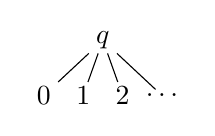
\begin{tikzpicture}[baseline=(root.base),level distance=7mm,inner ysep=0.5mm,sibling distance=5mm]
\node (root) {$q$}
child {node {$0$}}
child {node {$1$}}
child {node {$2$}}
child {node {$\ldots$}};
\end{tikzpicture}
\end{center}

Then the base type \texttt{exp} is interpreted by the flat game
$\nat$ over the previous arena where the set of valid position is:
$$P_N = \{ \epsilon, q \} \union \{ qn \ | \ n \in \omega \}$$


In this game, there is only one question: the initial O-question. P
can then answer by playing a natural number $i \in \omega$. There
are only two kinds of strategies on this arena:
\begin{itemize}
\item the empty strategy where P never answer the initial question. This corresponds to a non terminating computation;
\item the strategies where P answers by playing a number $n$. This models a numerical constant of the language.
\end{itemize}

Given the interpretation of base types, we define the interpretation
of $A\rightarrow B$ by induction:
$$\sem{A \rightarrow B} = \sem{A} \Rightarrow \sem{B}$$

where the operator $\Rightarrow$ denotes the game construction $!A
\multimap B$ i.e. the exponential object of the cartesian closed
category $\mathcal{C}$.



Variables are interpreted by projection:
$$\sem{x_1 : A_1, \ldots, x_n:A_n \vdash x_i : A_i} = \pi_i : \sem{A_i} \times \ldots \times \sem{A_i} \times \ldots \times \sem{A_n} \rightarrow  \sem{A_i}$$

The abstraction $\Gamma \vdash \lambda x :A.M : A \rightarrow B$ is
modeled by a strategy on the arena $\sem{\Gamma} \rightarrow
(\sem{A}\Rightarrow\sem{B})$. This strategy is obtained by using the
currying operator of the cartesian closed category:
$$\sem{\Gamma \vdash \lambda x :A.M : A \rightarrow B} = \Lambda( \sem{\Gamma, x :A \vdash M : B})$$

The application $\Gamma \vdash M N$ is modeled using the evaluation
map $ev_{A,B} : (A\Rightarrow B)\times A \rightarrow B$:

$$\sem{\Gamma \vdash M N} = \langle \sem{\Gamma \vdash M, \Gamma \vdash N} \rangle \fatsemi ev_{A,B}$$


\subsubsection{\pcf\ fragment}

We now show how to model \pcf\ constructs in the game semantics
setting. In the following, each sub-arena of a game is tagged so that it is possible to distinguish identical arenas
occurring in different components of the game. Moves are also tagged (in the exponent) so that it is possible
to identify the arena component in which the move belongs. We will
omit the pointers in the play when there is no ambiguity.

The successor arithmetic operator is modeled by the following
strategy on the arena $\nat^1 \Rightarrow \nat^0$:
$$\sem{\texttt{succ}} = \prefset^{\sf even} \{q^0 \cdot q^1 \cdot n^1 \cdot (n+1)^0\ |\ n \in \nat \}$$
where $\prefset^{\sf even} X$ denotes the set consisting of the prefixes of even length of plays of $X$.

The predecessor arithmetic operator is denoted by the strategy
$$\sem{\texttt{pred}} = \prefset^{\sf even} \left( \{q^0 \cdot q^1 \cdot n^1 \cdot (n-1)^0\ |\ n >0 \} \union \{ q^0 \cdot q^1 \cdot 0^1 \cdot 0^0 \} \right)$$

Then given a term $\Gamma \vdash \texttt{succ }M : \texttt{exp}$ we
define:
$$\sem{\Gamma \vdash \texttt{succ } M : \texttt{exp}} = \sem{\Gamma \vdash M} \fatsemi \sem{\texttt{succ}} $$
$$\sem{\Gamma \vdash \texttt{pred } M : \texttt{exp}} = \sem{\Gamma \vdash M} \fatsemi \sem{\texttt{pred}} $$


The conditional operator is denoted by the following strategy on the
arena $\nat^3 \times \nat^2 \times \nat ^1 \Rightarrow \nat^0$:
$$\sem{\texttt{cond}} = \prefset^{\sf even}
    \{ q^0 \cdot q^3 \cdot 0 \cdot q^2 \cdot n^2 \cdot n^0 \ | \ n \in \nat \}
    \union
    \prefset^{\sf even}  \{ q^0 \cdot q^3 \cdot m \cdot q^2 \cdot n^2 \cdot n^0 \ | \ m >0, n \in \nat \}
    $$


Given a term $\Gamma \vdash \texttt{cond}\ M\ N_1\ N_2$ we define:
$$\sem{\Gamma \vdash \texttt{cond}\ M\ N_1\ N_2} =
\langle \sem{\Gamma \vdash M}, \sem{\Gamma \vdash N_1}, \sem{\Gamma
\vdash N_2} \rangle \fatsemi \sem{\texttt{cond}}$$


The interpretation of the \texttt{Y} combinator is a bit more
complicated.

Consider the term $\Gamma \vdash M : A \rightarrow A$, its semantics
$f$ is a strategy on $\sem{\Gamma} \times \sem{A} \rightarrow
\sem{A}$. We define the chain $g_n$ of strategies on the arena
$\sem{\Gamma} \rightarrow \sem{A}$ as follows:
\begin{eqnarray*}
g_0 &=& \perp \\
g_{n+1} &=&  F(g_n) = \langle id_{\sem{\Gamma}}, g_n\rangle \fatsemi f
\end{eqnarray*}

where $\perp$ denotes the empty strategy $\{ \epsilon \}$.

It is easy to see that the $g_n$ forms a chain. We define
$\sem{\texttt{Y} M}$ to be the least upper bound of the chain $g_n$
i.e. the  least fixed point of $F$. Its existence is guaranteed by
the fact that the category of games is cpo-enriched.

Since all the strategies that we have given are innocent and
well-bracketed, the game model of \pcf\ can be interpreted in any of
the four categories $\mathcal{C}$, $\mathcal{C}_i$, $\mathcal{C}_b$,
$\mathcal{C}_{ib}$.



\subsection{Full-abstraction of \pcf}
In this section we state the full abstraction result proved in
\cite{abramsky94full} and \cite{hylandong_pcf}.


\subsubsection{Observational preorder}

A context denoted $C[-]$ is a term containing a hole denoted by $-$.
If $C[-]$ is a context then $C[M]$ denotes the term obtained after
replacing the hole by the term $M$. $C[M]$ is well-formed provided
that $M$ has the appropriate type. Remark: this capture-permitting
substitution must be distinguished from the capture-free
substitution which is denoted by $M[N/x]$ for any two terms $M$ and
$N$.

We say that two programs are observationally equivalent if they
can be safely interchanged in any program context.
\begin{definition}[Observational preorder]
We define the relation on terms $\obspre$ as follows: let $M$ and $N$ be two closed terms of the same type then:
\begin{eqnarray*}
M \obspre N &\iff& \parbox{10cm}{for all context $C[-]$ such that
                $C[M]$ and $C[N]$ are well-formed closed term of type \texttt{exp},
                    $C[M] \eval$ implies $C[N] \eval$}
\end{eqnarray*}
The observational equivalence relation, denoted by $\obseq$, is defined to be the reflexive closure of $\obspre$.
\end{definition}


\subsubsection{Soundness and adequacy}
A model of a programming language is said to be \emph{sound} or
\emph{inequationally sound} if whenever the denotation of two
programs are equal then the two programs are observationally
equivalent, or more formally if for any closed terms $M$ and $N$ of
the same type:
$$ \sem{M} \subseteq \sem{N} \imp M \obspre N.$$

In a way, soundness is the minimum one can require for a model of
programming language: it guarantees that we can reason about the
program by manipulating the object of the denotational model.

It can be shown that the game model of \pcf\ is sound for evaluation
and computationally adequate. These two properties imply the
soundness of the game model:

We said that the evaluation relation $\eval$ is sound if the
denotation is preserved by evaluation:
\begin{lemma}[Soundness of evaluation]
\label{lem:evalsoundness}
 Let $M$ be a PCF term then
$$M \eval V \quad \imp \quad \sem{M} = \sem{V}.$$
\end{lemma}

\begin{definition}[Computable terms] \
\begin{itemize}
\item A closed term $\vdash M$ of base type is computable if $\sem{M} \neq \bot$
implies $M \eval$.
\item A higher-order closed term $\vdash M : A\rightarrow B$ is computable if $M N$ is computable for any computable closed term $\vdash  N:A$.
\item An open term $x_1 : A_1, \ldots, x_n : A_n \vdash M : A\rightarrow B$ is computable if $\vdash M [N_1/x_1, \ldots N_n/x_n]$ is computable
for all computable closed terms $N_1:A_1, \ldots, N_n:A_n$.
\end{itemize}
\end{definition}

A model is \emph{computationally adequate} if all
terms are computable.
\begin{lemma}[Computational adequacy]
\label{lem:computadequacy}
The game model of PCF is
computationally adequate.
\end{lemma}
We refer the reader to \cite{abramsky:game-semantics-tutorial} for
the proofs.

Inequational soundness follows from the last two lemmas:
\begin{proposition}[Inequational soundness]
\label{prop:ineqsoundness} Let $M$ and $N$ be two closed terms then
$$\sem{M} \subseteq \sem{N} \implies  M \obspre N $$
\end{proposition}
\begin{proof}
  Suppose that $\sem{M} \subseteq \sem{N}$ and $C[M] \eval$ for some context $C[-]$. Then by compositionality of game semantics we also have
  $C[\sem{M}] \subseteq C[\sem{N}]$.
  Lemma \ref{lem:evalsoundness} gives $\sem{C[M]} \neq \bot$, therefore $\sem{C[N]} \neq \bot$.
  Lemma \ref{lem:computadequacy} then implies that $C[N] \eval$.
  Hence $M \obspre N$.
\end{proof}

\subsubsection{Definability}

We will now consider only strategies that are innocent and
well-bracketed which means that we work in the category
$\mathcal{C}_{ib}$.

The compact morphisms of the category $\mathcal{C}_{ib}$ are those
with finite view-function. The definability result says that every
compact element of the model is the denotation of some term.

The economical syntax of \pcf\ prevents us from stating this result
directly: we need to consider an extension of \pcf\ with some
additional constants. Indeed, there are strategies that are not the
denotation of any term in \pcf, for instance the ternary conditional
strategy : this strategy denotes the computation that tests the
value of its first parameter, if it is equal to zero or one then it
returns the value of the second or third parameter respectively,
otherwise it returns the value of the fourth parameter. This
strategy is illustrated by the left diagram on the next figure.

It is possible to simulate this computation in \pcf\ using the
conditional operator. For instance the term $T_3 = \texttt{cond}\ M\
N_1 (\texttt{cond}\ (\texttt{pred } M)\  N_2\ N_3)$ has the desired
operational semantics. The game semantics denotation of
$T_3$, however, is not given by the ternary conditional strategy. It is
instead given by the right diagram on the following figure.
$$
\begin{array}{ccccccccc}
!\bf N & \otimes & !\bf N & \otimes & !\bf N & \otimes & !\bf N & \multimap & !\bf N \\
&&&&&&&&q \\
q \\
0 \\
&& q \\
&& n \\
&&&&&&&&n \\
\hline
&&&&&&&&q \\
q \\
1 \\
&&&& q \\
&&&& n \\
&&&&&&&&n \\
\hline
&&&&&&&&q \\
q \\
m>1 \\
&&&&&& q \\
&&&&&& n \\
&&&&&&&&n \\
\end{array}
\hspace{0.3cm}
\begin{array}{ccccccccc}
!\bf N & \otimes & !\bf N & \otimes & !\bf N & \otimes & !\bf N & \multimap & !\bf N \\
&&&&&&&&q \\
q \\
0 \\
&& q \\
&& n \\
&&&&&&&&n \\
\hline
&&&&&&&&q \\
q \\
1 \\
q \\
0 \\
&&&& q \\
&&&& n \\
&&&&&&&&n \\
\hline
&&&&&&&&q \\
q \\
m>1 \\
q \\
m-1>0 \\
&&&&&& q \\
&&&&&& n \\
&&&&&&&&n \\
\end{array}
$$

To overcome this deficiency we add a family of terms to \pcf: the
$k$-ary conditionals:
$$ \texttt{case}_k\ N\ N_1\ N_2\ \ldots\ N_k$$
with the desired operational semantics:
$$ \rulef{M \eval i \quad N_{i+1} \eval V}{\texttt{case}_k\ N\ N_1\ N_2\ \ldots\ N_k\ \eval V}\ i \in \{0, \ldots,k-1\}.$$
The denotation of this term is given by the first strategy illustrated above.
The extended language is called \pcf'.

We can now prove the definability result:
\begin{proposition}[Definability]
\label{prop:definability} Let $A$ be a PCT type and $\sigma$ be a compact innocent and well-bracketed
strategy on $A$. There exists a PCF term $M$ such that $\sem{M} = \sigma$.
\end{proposition}

Note that definability is proved for \pcf' and not for \pcf.
Nevertheless, \pcf' is a conservative extension of \pcf: if $M$ and
$N$ are terms such that for any \pcf-context $C[-]$, $C[M] \eval
\imp C[N] \eval$ then the same is true for any \pcf'-context. This
is because $\texttt{case}_k$ constructs can be ``simulated'' in
\pcf, for instance $\texttt{case}_3$ can be replaced by the \pcf\
term $T_3$ which shares the same operational semantics.

This observation will allow us to use definability in \pcf' to
prove the full-abstraction of \pcf.


\subsubsection{Full abstraction}

Full abstraction of \pcf\ cannot be stated directly in the category $\mathcal{C}_{ib}$. Instead we need to consider the quotiented category
$\mathcal{C}_{ib}/\lesssim_{ib}$.

First we need to show that $\mathcal{C}_{ib}/\lesssim_{ib}$ is a
model of \pcf. $\mathcal{C}_{ib}/\lesssim_{ib}$ is a posset-enriched
cartesian closed category. The game semantics of the basic types and
constants of \pcf\ can be transposed from $\mathcal{C}_{ib}$ to
$\mathcal{C}_{ib}/\lesssim_{ib}$. Unfortunately it is not known
whether $\mathcal{C}_{ib}/\lesssim_{ib}$ is enriched over the
category of CPOs. However it can be proved that it is a rational
category \citep{abramsky94full} and this suffices to ensure that
$\mathcal{C}_{ib}/\lesssim_{ib}$ is indeed a model of \pcf. The full
abstraction of the game model then follows from proposition
\ref{prop:ineqsoundness} and \ref{prop:definability}:
\begin{theorem}[Full abstraction]
Let $M$ and $N$ be two closed IA-terms.
$$\sem{M} \precsim_{ib} \sem{N} \ \iff \ M \obspre N$$
where $\precsim_{ib}$ denotes the intrinsic preorder of the category $\mathcal{C}_{ib}$.
\end{theorem}

\section{The fully abstract game model for Idealized Algol (\ialgol)}

We now extend the work of the previous section to the language
\ialgol, an imperative extension of \pcf. We start by giving the
syntax and operational semantics of the language, we then describe
the game model which was introduced in \cite{abramsky99full}.
Finally we will state the full abstraction result for the game
model.

\subsection{The syntax of \ialgol}
IA is an extension of \pcf\ introduced by J.C. Reynold in
\cite{Reynolds81}. It adds imperative features such as local
variables and sequential composition. On top of \texttt{exp}, \pcf\
has two new types: \texttt{com} for commands and \texttt{var} for
variables. There is a constant \texttt{skip} of type \texttt{com}
which corresponds to the command that does nothing.

Commands can be composed using the sequential composition operator
$\texttt{seq}_A$: suppose that $M$ and $N$ are of type \texttt{com}
and $A$ respectively then they can be composed to form the term $S =
\texttt{seq}_A M N : \texttt{com}$. $S$ denotes program that
executes $M$ until it terminates and then behaves like $N:A$. If $A
= \texttt{exp}$ then the expression is allowed to have a side-effect
and $S$ returns the expression computed by $N$, if $A =
\texttt{com}$ then the command $N$ is executed after $M$. We say
that the language has \emph{active expressions} to indicate the
presence of the sequential operator $\texttt{seq}_{\iaexp}$ in the
language.


Local variables are
declared using the \texttt{new} operator, variable content is altered
using \texttt{assign} and retrieved using \texttt{deref}.

In addition IA has the constant \texttt{mkvar} that can be used to
create a particular kind of variables. The \texttt{mkvar} operator
works in an object oriented fashion: it takes two arguments, the
first one is a function (called the acceptor) that affects a value
to the variable and the second argument is an expression that
returns a value from the variable. This mechanism is similar to
the ``set/get'' object programming paradigm used by C++ programmers.

Variables created with \texttt{mkvar} are less constrained than the
variables created with \texttt{new}. Indeed, variables created with
\texttt{new} act like memory cells, they obey the following rule:
the value read from the variable is always the last value that has
been assigned to it. This rule does not apply to variables created
with \texttt{mkvar}. For instance the variable:
$$\texttt{mkvar}\ (\lambda v.\texttt{skip})\ 0$$
will always return $0$ even if another number has been assigned it.


One may think that this addition to the language is artificial, however the full abstraction result of the game model of IA relies upon this addition.\footnote{McCusker showed in \cite{mccusker2001} that the game model of IA with \iamkvar\ which is fully abstract with respect to the observational preorder is also fully abstract for the language without \iamkvar\, but for observational equivalence only. Hence the model is equationally but not inequationally fully abstract for IA without \iamkvar .}

The set of additional formations rules completing those of \pcf\ are
given in table \ref{tab:ia_formrules}. Judgements are of the form
$\Gamma \vdash M : A$. If $\Gamma = \emptyset$ then we say that $M$
is a closed term.

\begin{table}[htbp]
$$ \rulef{\Gamma \vdash M : \texttt{com} \quad \Gamma \vdash N :A}
    {\Gamma \vdash \texttt{seq}_A \ M\ N\ : A} \quad A \in \{ \texttt{com}, \texttt{exp}\}$$

$$ \rulef{\Gamma \vdash M : \texttt{var} \quad \Gamma \vdash N : \texttt{exp}}
    {\Gamma \vdash \texttt{assign}\ M\ N\ : \texttt{com}}
\qquad
 \rulef{\Gamma \vdash M : \texttt{var}}
    {\Gamma \vdash \texttt{deref}\ M\ : \texttt{exp}}$$

$$ \rulef{\Gamma, x : \texttt{var} \vdash M : A}
    {\Gamma \vdash \texttt{new } x \texttt{ in } M} \quad A \in \{ \texttt{com}, \texttt{exp}\}$$

$$ \rulef{\Gamma \vdash M_1 : \texttt{exp} \rightarrow \texttt{com} \quad \Gamma \vdash M_2 : \texttt{exp}}
    {\Gamma \vdash \texttt{mkvar } M_1\ M_2\ : \texttt{var}}$$

\caption{Formation rules for IA terms}
\label{tab:ia_formrules}
\end{table}


\subsection{Operational semantics of \ialgol}

The operational semantics of IA is given in a slightly different
form compared to \pcf. Instead of giving the semantics for closed
terms we consider terms whose free variables are all of type
\texttt{var}. Terms are ``closed'' by means of stores. A store is a
function mapping free variables of type \texttt{var} to natural
numbers. Suppose $\Gamma$ is a context containing only variables of
type \texttt{var}, then we say that $\Gamma$ is a
\texttt{var}-context. A store with domain $\Gamma$ is called a
$\Gamma$-store. The notation $s\ |\ x \mapsto n$ refers to the store
that maps $x$ to $n$ and acts according to the store $s$ otherwise.

%%%% The following is poorly written:
%
%In \pcf, the evaluation rules were given for closed terms only.
%Suppose that we proceed the same way for IA and consider the
%evaluation rule for the $\texttt{new}$ construct: the conclusion is
%$\texttt{new } x:=0 \texttt{ in } M$ and the premise is an
%evaluation for a certain term constructed from $M$, more precisely
%the term $M$ where \emph{some} occurrences of $x$ are replaced by
%the value $0$. Because of the presence of the \texttt{assign}
%operator, we cannot simply replace all the occurrences of $x$ in $M$
%(the required substitution is  more complicated than the
%substitution used for beta-reduction).


The canonical forms for IA are given by the grammar:
$$ V ::= \texttt{skip}\ |\ n\ |\ \lambda x. M\ |\ x\ |\  \texttt{mkvar}\ M\ N$$

where $n \in \nat$ and $x: \texttt{var}$.


In \ialgol, a program is a term together with a $\Gamma$-store such
that $\Gamma \vdash M : A$. The evaluation semantics is expressed by
the judgment form:
$$s,M \eval s', V$$
where $s$ and $s'$ are $\Gamma$-stores, $V$ is a canonical form and $\Gamma \vdash V : A$.

The operational semantics for IA is given by the rule of \pcf\ (table \ref{tab:bigstep_pcf})
together with the rules of table \ref{tab:bigstep_ia} where the following abbreviation is used:
$$ \rulef{M_1 \eval V_1 \quad M_2 \eval V_2}{M \eval V} \qquad \mbox{for} \qquad
  \rulef{s,M_1 \eval s',V_1 \quad s', M_2 \eval s'',V_2 }{s,M \eval s'',V}
$$


\begin{table}[htbp]
$$\mbox{\textbf{Sequencing }}
    \rulef{M \eval \iaskip \quad N \eval V}{\texttt{seq } M\ N \eval V}
$$

$$\mbox{\textbf{Variables }}
    \rulef{s,N \eval s',n \quad s',M \eval s'',x}{s, \iaassign\ M\ N \eval (s''\ |\ x \mapsto n),\iaskip}
\qquad
    \rulef{s,M \eval s',x }{s, \iaderef\ M \eval s',s'(x)}$$

$$\mbox{\texttt{\textbf{mkvar}}}
    \rulef{N \eval n \quad M \eval \texttt{mkvar}\ M_1\ M_2 \quad M_1\ n \eval \iaskip}
    {\iaassign\ M\ N \eval \iaskip}
\qquad
    \rulef{N \eval \texttt{mkvar } M_1\ M_2 \quad M_2\ \eval n}
    {\iaderef\ M \eval n}
$$

$$\mbox{\textbf{Block}}
    \rulef{(s\ |\ x \mapsto 0),M \eval (s'\ |\ x \mapsto n),V }
    {s, \texttt{new } x \texttt{ in } M \eval s',V}
$$

\label{tab:bigstep_ia}
\caption{Big-step operational semantics of IA}
\end{table}

\subsection{Small-step semantics of \ialgol}
\label{subsec:smallstep_ia}
The previous section defined the operational semantics of
\ialgol\ using a big step semantics. Equivalently, we can define it using a small-step semantics.
The reduction rules of the small-step semantics are of the form $s,e
\rightarrow s',e'$ where $s$ and $s'$ denotes the stores and $e$ and
$e'$ denotes \ialgol\ expressions.

The reduction rules are the following:
\begin{itemize}
\item the $\beta$-reduction;
\item reduction rules for \pcf\ constants:
\begin{eqnarray*}
\pcfsucc\ n &\rightarrow& n+1 \\
\pcfpred\ n+1 &\rightarrow& n \\
\pcfpred\ 0 &\rightarrow& 0 \\
\pcfcond\ 0\ N_1 N_2 &\rightarrow& N_1 \\
\pcfcond\ n+1\ N_1 N_2 &\rightarrow& N_2 \\
Y\ M &\rightarrow& M (Y M)
\end{eqnarray*}
\item reduction rules for \ialgol\ constants:
\begin{eqnarray*}
\iaseq\ \iaskip\  M &\rightarrow& M \\
s, \ianewin{x}\ M &\rightarrow& (s|x\mapsto 0), M \\
s, \iaassign\ x\ n &\rightarrow& (s|x\mapsto n), \iaskip \\
s, \iaderef\ x &\rightarrow& s, s(x) \\
\iaassign\ (\iamkvar M N)\ n &\rightarrow& M n \\
\iaderef\ (\iamkvar M N) &\rightarrow& N
\end{eqnarray*}
\end{itemize}

Redex can also be reduced when they occur as subexpressions within a
larger expression. We make use of evaluation contexts to indicate
when such reduction can happen. Evaluation contexts are given by the
following grammar:
\begin{eqnarray*}
E[-] &::=& - |\ E N\ |\ \pcfsucc\ E\ |\ \pcfpred\ E\ |\ \pcfcond\ E\ N_1\ N_2\ |\ \\
&&    \iaseq\ E\ N\ |\ \iaderef\ E\ |\ \iaassign\ E\ n\ |\ \iaassign\ M\ E \ |\ \\
&&    \iamkvar\ M\ E\ |\ \iamkvar\ E\ M\ |\ \ianewin{x}\ E  .
\end{eqnarray*}

The small-step semantics is completed with following rule:
$$ \rulef{M \rightarrow N}{E[M] \rightarrow E[N]} $$

\subsection{Game model of \ialgol}

All the strategies used to model \pcf\ are well-bracketed and
innocent. On the other hand, to obtain a model of IA we need to
introduce strategies that are not innocent. This is necessary to
model memory cell variable created with the \texttt{new} operator.
The intuition is that a cell needs to remember the last value which
was written in it in order to be able to return it when it is read,
and this can only be done by looking at the whole history of moves,
not only those present in the P-view. Hence we now consider the
categories $\mathcal{C}$ and $\mathcal{C}_b$.

\subsubsection{Base types}

The type \texttt{com} is modeled by the flat game with a single initial question \texttt{run} and a single answer
\texttt{done}. The idea is that O can request the execution of a command by playing \texttt{run}, P then executes the command
and if it terminates, acknowledges it by playing \texttt{done}.

The variable type \texttt{var} is modeled by the game $\tt{com^{\bf
N} \times exp}$ illustrated below:
\begin{center}
\begin{tikzpicture}[baseline=(root.base),level distance=10mm,inner ysep=0.5mm]%,sibling distance=5mm
 \node{\tt{ok}}  [grow'=up]
    child {node {$\tt{write}_0$}}
    child {node {$\tt{write}_1$}}
    child {node {$\tt{write}_2$}}
    child {node {$\ldots$}}
;
\draw +(5,+10mm) node {\tt{read}}
    child {node {$0$}}
    child {node {$1$}}
    child {node {$2$}}
    child {node {$\ldots$}}
;
\end{tikzpicture}
\end{center}

\subsubsection{Constants}

\texttt{skip} is interpreted by the strategy $\{ \epsilon, \iarun
\cdot \iadone \}$. The sequential composition $\tt{seq_{exp}}$ is
interpreted by the following strategy:
$$
\begin{array}{ccccc}
!\iacom & \otimes & ! \iaexp & \stackrel{\iaseq_{\iaexp}}{\multimap} & \iaexp\\
&&&&q\\
\iarun\\
\iadone\\
&&q\\
&&n\\
&&&&n
\end{array}
$$

Assignment \iaassign\ and dereferencing \iaderef\ are denoted  by the
following strategies (left and right respectively):
$$
\begin{array}{ccccc}
!\iavar & \otimes & ! \iaexp & \stackrel{\iaassign}{\multimap} & \iacom\\
&&&&q\\
&&q\\
&&n\\
\iawrite_n\\
\iaok\\
&&&&\iadone
\end{array}
\hspace{3cm}
\begin{array}{ccccc}
!\iavar & \stackrel{\iaderef}{\multimap} & \iaexp\\
&&q\\
\iaread\\
n\\
&&n
\end{array}
$$

\iamkvar\ is modeled by the paired strategy $\langle \iamkvar_{acc} , \iamkvar_{exp}
\rangle$ where $\iamkvar_{acc}$ and $\iamkvar_{exp}$ are the following strategies:
$$
\begin{array}{ccccccc}
!(!\iaexp & \multimap & \iacom) & \otimes & !\iaexp & \stackrel{\iamkvar_{acc}}{\multimap} & \iacom^\omega\\
&&&&&&\iawrite_n\\
&&\iarun\\
q\\
n\\
&&\iadone \\
&&&&&&\iaok
\end{array}
\hspace{0.2cm}
\begin{array}{ccccccc}
!(!\iaexp & \multimap & \iacom) & \otimes & !\iaexp & \stackrel{\iamkvar_{exp}}{\multimap} & \iaexp\\
&&&&&&\iaread\\
&&&&q\\
&&&&n\\
&&&&&&n \\ \  \\ \
\end{array}
$$


The strategies used until now are all innocent. In order to model
the \ianew\ operator, we need to introduce non-innocent strategies,
sometimes called \emph{knowing strategies}. We define the knowing
well-bracketed strategy $cell : I \multimap !\iavar$ that models a
storage cell: it responds to \iawrite\ with \iaok\ and responds to
\iaread\ with the last value written or $0$ if no value has yet been
written.

Consider the term $\Gamma,x:\iavar \vdash M : A$ modeled by
$\sem{M}$ then the term
 $\Gamma \vdash \ianewin{x}\ M : A$  will be modeled by the strategy $(id_{\sem{\Gamma}} \otimes cell) \fatsemi \sem{M}$ on the game
 $!\Gamma \multimap \iacom$.

\subsection{Full abstraction of \ialgol}

We now state the full abstraction result. All the details are
omitted, the reader is referred to
\cite{abramsky:game-semantics-tutorial,AM97a} for the proofs.

\subsubsection{Inequational soundness}

The inequational soundness result can be also proved for \ialgol.
Proving soundness of the evaluation requires a bit more work than in
the \pcf\ case because the store needs to be made explicit. Also, we
need to define an appropriate notion of \emph{computable term} that
takes into account the presence of stores in the evaluation
semantics. It is possible to prove that the model is computational
adequate. The inequational soundness then follows from evaluation
soundness and computational adequacy.

%\begin{lemma}[Soundness for IA terms] Let $\Gamma \vdash M : A$ be an IA term and a $\Gamma$ store $s$.
%If $s,M \eval s',V$ then the plays of $\sem{s,M} : I \multimap A
%\otimes !\Gamma$ which begin with a move of $A$ are identical to
%those of $\sem{s',V}$.
%\end{lemma}

\begin{proposition}[Inequational soundness]
\label{prop:ia_ineqsoundness} Let $M$ and $N$ be two IA closed terms then
$$\sem{M} \subseteq \sem{N} \implies  M \obspre N $$
\end{proposition}

\subsubsection{Definability}

The proof of definability is based on a factoring argument: strategies in
$\mathcal{G}_b$ can all be obtained by composing the non-innocent strategy $cell$ with an innocent strategy.
The strategy $cell$ can therefore be viewed as a generic non-innocent strategy. Using this factorization argument,
it is possible to prove the definability result:
\begin{proposition}[Definability]
\label{prop:ia_definability} Let $\sigma$ be a compact well-bracketed
strategy on a game $A$ denoting a IA type. There is an IA-term $M$ such
that $\sem{M} = \sigma$.
\end{proposition}

\subsubsection{Full abstraction}

Full abstraction for the model $\mathcal{C}_b$ is a consequence of proposition
\ref{prop:ia_ineqsoundness} and \ref{prop:ia_definability}:
\begin{theorem}[Full abstraction]
Let $M$ and $N$ be two closed IA-terms.
$$\sem{M} \precsim_b \sem{N} \ \iff \ M \obspre N$$
where $\precsim_b$ denotes the intrinsic preorder of the category
$\mathcal{C}_b$.
\end{theorem}


\section{Algorithmic game semantics}

After the resolution of the ``Full Abstraction of \pcf'' problem, game semantics has become a very successful paradigm in fundamental computer science. It has permitted to give full abstract semantics for a variety of programming languages. More recently, game semantics has emerged as a new approach to program verification and program analysis. In particular in the paper \cite{ghicamccusker00}, the authors considered a fragment of Idealized Algol for which the game semantics of programs can be expressed simply using regular expressions. In this setting, observational equivalence of programs becomes decidable. Consequently, numbers of interesting verification problems become solvable. This development opened up a new direction
of research called \emph{Algorithmic game semantics}.

\subsection{Characterisation of observational equivalence}

In \citep{AM97a} it is shown that observational equivalence of IA is characterised by the equality of the set of complete plays.

A play of a game is \emph{complete} if it is maximal and all
question have been answered. A game is \emph{simple} if the complete plays are exactly those in which the initial question has been answered. It can be shown that for any IA type $T$, $\sem{T}$ is a simple game. The following characterisation theorem holds for simple games:
\begin{theorem}[Characterisation Theorem for Simple Game (Abramsky, McCusker 1997)]
Let $\sigma$ and $\tau$ be strategies on a simple game $A$ then:
$$\sigma \leq \tau \iff \textit{comp}(\sigma) \subseteq \textit{comp}(\tau)$$
\end{theorem}
Therefore the game semantics of an IA term is fully determined by the set of complete plays of the strategy denoting it.

\subsection{Finitary fragments of Idealized algol}
We introduce
some fragments of the language \ialgol. Firstly, \emph{Finitary
Idealized Algol} denotes the recursion-free sub-fragment of \ialgol\
over finite ground types (i.e. $\nat$ is replaced by the set $0..max$ for some
fixed value $max$).

\begin{definition}[$i$th order \ialgol\ term]
A term $\Gamma \vdash M:T$ of finitary Idealized algol is an $i$th-order term if any sequent $\Gamma' \vdash N:A$ appearing
in the typing derivation of $M$ is such that $\ord{A} \leq i$ and all the variables in $\Gamma'$ are of order strictly less than $i$.
\end{definition}

$\ialgol_i$ denotes the fragment of finitary Idealized Algol
consisting of the collection of $i$th-order terms.

$\ialgol_i + \textsf{while}$ denotes the fragment $\ialgol_i$ augmented with
primitive recursion : the formation rules of $\ialgol_i + \textsf{while}$  are those
of $\ialgol_i$ together with the following rule:
$$  \rulef{\Gamma \vdash M : \iabool \qquad \Gamma \vdash N : \iacom}{\Gamma \vdash \iawhile\ M \iado\ N : \iacom } \quad \mbox{where } \forall x \in \Gamma : \ord{x} < i $$

Finally $\ialgol_i + \textsf{Y}_j$ where $j
< i$ denotes the fragment $\ialgol_i$ augmented with a set of
fixed-point iterators $\textsf{Y}_A : (A\rightarrow A ) \rightarrow
A$ for any type $A$ of order $j$ at most. The formation rules of $\ialgol_i + \textsf{Y}_j$  are those
of $\ialgol_i$ together with the following rule:
$$  \rulef{\Gamma \vdash \lambda x . M : A\rightarrow A}{\Gamma \vdash Y_A M : A} \quad \mbox{where } \forall x \in \Gamma : \ord{x} < i
                                                                            \mbox{ and } \ord{A} \leq j $$

We recall the observational equivalence decision problem: given two
$\beta$-normal forms $M$ and $N$ in a given fragment of \ialgol,
does $M \approx N$ hold?

This problem has been investigated and decidability results have
been obtained for a complete class of fragments of Idealized Algol.
These results help us to understand the limits of Algorithmic Game
Semantics. We now present briefly those results.

\subsubsection{The order-\texorpdfstring{$2$}{2} fragment of \ialgol}
In \cite{ghicamccusker00}, the authors show that in the $\ialgol_2$ fragment,
the set of complete plays are representable by extended regular languages.

\begin{lemma}[Ghica and McCusker 2000]
For any IA$_2$-term $\Gamma \vdash M : T$, the set of complete
plays of $\sem{\Gamma \vdash M : T}$ is regular.
\end{lemma}
Since equivalence of regular expression is decidable, this shows
decidability of observational equivalence of $\ialgol_2$-terms. In
the same paper they show that the same result holds for the
$\ialgol_2 +\textsf{while}$ fragment.

In \cite{Ong02}, it is shown that observational equivalence is
undecidable for $\ialgol_2 + \textsf{Y}_1$.


\subsubsection{Other fragments of IA}

Observational equivalence is decidable for $\ialgol_3$. This is
proved in \cite{Ong02} by reduction to the \emph{Deterministic
Push-down Automata Equivalence} problem. Unfortunately, this result
cannot be extended beyond order $3$: Murawski showed in
\cite{murawski03program} that the problem is undecidable for
$\ialgol_i$ with $i\geq4$.

In \citep{DBLP:conf/fossacs/MurawskiW05},
\citeauthor{DBLP:conf/fossacs/MurawskiW05} show decidability for $\ialgol_3 + \textsf{while}$. They also prove that for $\ialgol_3$ and $\ialgol_3 + \textsf{while}$ the problem lies in EXPTIME.

In \cite{DBLP:conf/icalp/MurawskiOW05} it is shown that
$\ialgol_i +Y_0$ for $i = 1, 2, 3$ is as difficult as the DPDA
equivalence problem. This problem is decidable
\citep{DBLP:journals/tcs/Senizergues01} but no complexity result is
known about it. We only know that it is primitive recursive
\citep{stirling02}.

\subsubsection{The complete classification}
\begin{center}
\begin{tabular}{rcccc}
Fragment  & pure & +while & +Y0 & +Y1 \\ \hline \hline
$\ialgol_0$ & PTIME & $\times^{(i)}$ & $\times$ & $\times$  \\
$\ialgol_1$ & coNP & PSPACE & DPDA EQUIV & $\times$ \\
$\ialgol_2$ & PSPACE & PSPACE & DPDA EQUIV & undecidable \\
$\ialgol_3$ &EXPTIME & EXPTIME & DPDA EQUIV & undecidable \\
$\ialgol_i, i \geq 4$  & undecidable & undecidable & undecidable
& undecidable
\end{tabular}
\vspace{12pt}

\emph{Notes}: The $\times$ symbol denotes undefined \ialgol\ fragments.
(i) Adding iteration to $\ialgol_0$ does not increase the power of the language since variables are forbidden in the language.
\end{center}

The coNP and PSPACE results are due to Murawski \citep{Mur04b}.
